\documentclass[10pt,letterpaper]{article}
\usepackage[T1]{fontenc}
\usepackage[utf8]{inputenc}
\usepackage{lmodern}
\usepackage[margin=0.88in]{geometry}
\usepackage{amsmath,amssymb,amsthm,mathtools}
\usepackage{graphicx,booktabs,tabularx,array,multirow}
\usepackage{algorithm,algpseudocode}
\usepackage{microtype}
\usepackage{xcolor,tikz,pgfplots}
\usetikzlibrary{arrows.meta,positioning,calc,shapes.geometric}
\pgfplotsset{compat=1.18}
\usepackage[round,authoryear]{natbib}
\usepackage[colorlinks=true,linkcolor=blue!55!black,citecolor=blue!55!black,urlcolor=blue!55!black]{hyperref}
\usepackage[nameinlink,capitalise,noabbrev]{cleveref}
\setlength{\parskip}{0.24em}
\setlength{\parindent}{1.2em}
\definecolor{methodblue}{RGB}{23,91,133}
\definecolor{methodteal}{RGB}{13,128,134}
\definecolor{methodorange}{RGB}{181,111,40}
\newtheorem{lemma}{Lemma}[section]
\newtheorem{proposition}[lemma]{Proposition}
\newtheorem{remark}[lemma]{Remark}
\newcommand{\R}{\mathbb{R}}
\newcommand{\sphere}{\mathbb{S}}
\newcommand{\cut}{\mathcal{C}}
\newcommand{\1}{\mathbf{1}}
\newcommand{\argmax}{\operatorname*{arg\,max}}
\newcommand{\sign}{\operatorname{sign}}
\newcommand{\GW}{\mathrm{GW}}
\newcommand{\HP}{\mathrm{HP}}
\newcommand{\meanRel}{\overline{\Delta}^{\mathrm{rel}}}
\newcommand{\sourcecode}[1]{\texttt{\detokenize{#1}}}
\title{\bfseries Seven Leading Max-Cut Rounding Protocols:\\
Algorithms, Derivations, Implementation Details, and a 71-Graph Empirical Comparison}
\author{Heriberto Espino-Montelongo\\
\small Universidad de las Am\'ericas Puebla}
\date{Research methods manuscript -- 10 November 2026\\
\small Working analysis; not a claim of a new approximation guarantee}
\begin{document}
\maketitle
\begin{abstract}
We provide an implementation-grounded, step-by-step mathematical explanation of seven protocols selected from the full Experiment025 and Experiment027 Max-Cut studies on the same 71 weighted G-set graphs. The selection rule is the equally weighted mean relative improvement, over the \emph{refined} Goemans--Williamson (GW) baseline, of the best signed cut obtained across 16 common starting normals. The seven leading protocols are Hyperplane Sweep, Angular Gain Greedy, Angular Margin Greedy, Angular Pair Greedy, Paired Spherical K-Means, EM--Gibbs, and Cut-aware K-Means. Their observed gains range from 0.2668\% to 0.3176\%. We derive the signed vertex-flip identity, an exact event-driven angular sweep, the geometric ranking rules and pairwise tangent construction, fixed-direction exact threshold optimization, spherical Lloyd updates, and the entropy-regularized Bernoulli/Gibbs mechanism. An important experimental qualification is that published rankings use subsequent common Flip/Kernighan--Lin/iterated-local-search refinement: they do \emph{not} isolate pure hyperplane rounding. The Experiment027 subset has independently audited 3,408 new and 2,272 comparator seed archives; the historical 18-method Experiment025 ranking is supported by a complete aggregate CSV but has not undergone the same independent archive-wide partition rescore. We distinguish conditional exactness from global optimality, method diversity from compute-matched superiority, and observed rank from inferential certainty.
\end{abstract}
\noindent\textbf{Keywords:} Max-Cut; SDP rounding; Goemans--Williamson; hyperplane search; angular greedy optimization; spherical K-Means; Gibbs sampling; reproducible experiments.

\tableofcontents
\clearpage

\section{Problem, notation, and the shared experimental design}\label{sec:problem}
\subsection{Signed Max-Cut on a fixed SDP-derived embedding}
Let $G=(V,E,w)$ be an undirected graph with $n=|V|$, $m=|E|$,
symmetric adjacency $W=(w_{ij})$, $W_{ii}=0$, and possibly negative
weights. Encode a binary partition by $\ell\in\{0,1\}^n$ or spins
$s_i=1-2\ell_i\in\{-1,+1\}$. The \emph{original signed} cut objective is
\begin{equation}\label{eq:cut}
\cut(s)=\sum_{\{i,j\}\in E}w_{ij}\1[s_i\ne s_j]
=\frac12\sum_{\{i,j\}\in E}w_{ij}(1-s_i s_j).
\end{equation}
A negative crossing edge \emph{reduces} this score.
In the SDP relaxation, $s_i s_j$ becomes a Gram entry $X_{ij}$,
subject to $X\succeq0$ and $X_{ii}=1$. The existing EVA-derived
factor $Y\in\R^{n\times p}$ has rows $y_i^\top$ and approximates
an SDP-feasible unit-diagonal Gram factorization $X=YY^\top$.
Every method in this paper uses the \emph{same frozen} $Y$;
no SDP/EVA problem has been solved anew.

Classical binary GW rounding samples $z\sim N(0,I_p)$,
normalizes $r=z/\|z\|_2$ and sets
\begin{equation}\label{eq:gw}
\ell_i^{\GW}(r)=\1[y_i^\top r>0],\quad
s_i^{\GW}=1-2\ell_i^{\GW},\quad
F(r)=\cut(s^{\GW}(r)).
\end{equation}
The repository's \sourcecode{FJ} and \sourcecode{GW-RR} labels both refer
to this one-hyperplane binary construction in the $k=2$ setting.
The classical guarantee for nonnegative-weight Max-Cut with a
suitable SDP optimum \citep{goemans1995} does \emph{not}
automatically apply to an approximate EVA factor on signed graphs.

\subsection{The signed single-vertex gain}
\begin{lemma}[Vertex-flip identity]\label{lem:flip}
For a spin assignment $s$, changing only the sign of vertex $i$
changes the original signed cut by
\begin{equation}\label{eq:flip}
g_i(s)=\cut(s^{\oplus i})-\cut(s)
=s_i\sum_j w_{ij}s_j=s_i(Ws)_i.
\end{equation}
\end{lemma}
\begin{proof}
Terms not incident to $i$ cancel. An incident edge's contribution
changes from $w_{ij}(1-s_i s_j)/2$ to
$w_{ij}(1+s_i s_j)/2$. The difference is $w_{ij}s_i s_j$;
summing gives \eqref{eq:flip}.
\end{proof}
After flipping $i$, a neighbor's gain changes by
$g_j\gets g_j-2w_{ij}s_i s_j$ using the spins before that flip.
The same identity supports exact hyperplane-crossing sweeps and
unrestricted graph label refinement, but the two uses are not
interchangeable.

\subsection{Raw rounding versus the common refinement}
For method $a$, graph $g$ and shared GW normal $r_{gt}$,
$t\in\{1,\ldots,16\}$, write $C^{\rm raw}_{gat}$ for
the objective immediately after \emph{method-specific rounding}.
In Experiment025/027, that partition then undergoes
\[
\boxed{\text{Round}\longrightarrow
\text{Flip (20 sweeps)}\longrightarrow
\text{KL (30 passes)}\longrightarrow
\text{ILS--KL (80 cycles, eight inner KL passes)}.}
\]
Settings are upper bounds, and the journal retains the
\emph{best} original-graph cut seen at any step, not simply
the final walker state. A discrete Flip/KL/ILS partition
need not be representable by a hyperplane in the original embedding.

The historical performance estimand is
\begin{equation}\label{eq:metric}
B_{ga}=\max_{1\le t\le16}C^{\rm final}_{gat},\qquad
R_a=\frac{100}{71}\sum_{g\in\mathcal G}
\frac{B_{ga}-B_{g,\GW}}{B_{g,\GW}},
\quad|\mathcal G|=71.
\end{equation}
All recorded refined GW denominators are positive.
This is an \emph{equally weighted graphwise best-of-16}
measure, not a one-start expectation or cut-per-second score.
Each method's raw step is separate from its final score.

\subsection{Selection, status and comparability}
Among the 18 Experiment025 protocols and three Experiment027
additions, the seven largest reported $R_a$ values were selected.
Experiment025 contains an aggregate of $71\times18\times16$
completed refined starts, but the full original 20,448
partition archives are \emph{not yet independently backed up
and rescored off VM} \citep{experiment025}. Experiment027
independently audits 3,408 new method--seed archives and
2,272 historical GW/Hyperplane Sweep comparators \citep{experiment027}.
Thus the pooled ranking is useful while its provenance depth
differs between studies.

The graph identity, archived EVA factor, 16 GW normals,
original signed objective and refinement policy were held
consistent. \emph{Matched starts do not mean equal algorithmic work}.
The historical confidence intervals use 30,000 graph bootstrap
resamples; the later audit uses 2,000. Seeds within a graph are
correlated, so the graph, not the seed, is the inference unit.

\begin{figure}[tb]
\centering
\begin{tikzpicture}[
  every node/.style={font=\footnotesize,align=center},
  step/.style={draw=methodblue!75,rounded corners=3pt,thick,fill=blue!5,
     minimum height=9mm,text width=31mm},
  arrow/.style={-{Latex[length=2.5mm]},thick,draw=methodblue},
  node distance=8mm]
\node[step] (embed) {Saved EVA vectors\\$Y\in\R^{n\times p}$};
\node[step,right=of embed] (round) {Method-specific\\rounding/initializer};
\node[step,right=of round] (raw) {Original signed\\raw cut};
\node[step,below=10mm of raw] (refine) {Flip $\to$ KL\\$\to$ ILS--KL};
\node[step,left=of refine] (final) {Best-ever\\refined cut};
\draw[arrow] (embed)--(round);
\draw[arrow] (round)--(raw);
\draw[arrow] (raw)--(refine);
\draw[arrow] (refine)--(final);
\node[draw=methodorange,rounded corners=2pt,fill=orange!7,
 text width=64mm,below=10mm of round] (note)
 {Only the \textbf{raw} cut measures what the geometric rounding method produced.};
\draw[-{Latex},methodorange,thick] (raw.south west) to[bend right=16] (note.east);
\end{tikzpicture}

\caption{The method-specific raw candidate and the common Flip/KL/ILS
pipeline are distinct experimental stages. The proposed future
geometry-only study would stop at the \emph{raw} cut, not at
the best after unrestricted label refinement.}
\label{fig:pipeline}
\end{figure}

\section{Method 1: Hyperplane Sweep}\label{sec:hyperplane}
\subsection{Mechanism: continuous normals, discrete partitions}
The implemented \texttt{hyperplane-sweep} method moves the normal of an origin-passing separating hyperplane, keeping the embedding $Y$ fixed. The current state is a unit normal $r\in\sphere^{p-1}$ and cut $\cut(s(r))$. A sweep is exact along a \emph{chosen} rotation path, not globally over every possible separating direction.

Choose a unit tangent $u$ with $u^\top r=0$ and set
\begin{equation}\label{eq:arc}
r(\theta)=r\cos\theta+u\sin\theta,\qquad -\pi/2<\theta<\pi/2.
\end{equation}
With $a_i=y_i^\top r$ and $b_i=y_i^\top u$, the only sign changes occur when $a_i\cos\theta+b_i\sin\theta=0$. In the open interval, $\cos\theta>0$, so for $b_i\ne0$ the crossing angle is
\begin{equation}\label{eq:angle}
\theta_i=\arctan(-a_i/b_i).
\end{equation}
If $b_i=0\ne a_i$ no crossing occurs; a zero projection along the entire path requires fixed tie handling. Vertices crossing at the same angle must be processed as a group. The signed gain formula \eqref{eq:flip} updates the score without recomputing every edge after each crossing.

\begin{proposition}[Exact fixed-arc search]\label{prop:arc}
Under exact arithmetic, sorting crossing events and updating the signed gains finds the best cut among the constant-partition open intervals of one specified semicircle, in $O(np+n\log n+m)$ time including the projections and sparse-edge updates.
\end{proposition}
\begin{proof}
There are at most $n$ crossings. Every open interval between consecutive crossings has an identical binary partition, so its cut is constant. Each vertex flips at most once; the incident-edge updates for all flips sum to $O(m)$. Sorting costs $O(n\log n)$ and projections cost $O(np)$. Taking the maximum of all visited interval values establishes the restricted optimum.
\end{proof}
The source independently reconstructs and checks the selected normal, partition, and original signed objective. If floating-point degeneracies prevent reconstruction, it retains the original cut rather than asserting an unattainable event score.
\begin{figure}[tb]
\centering
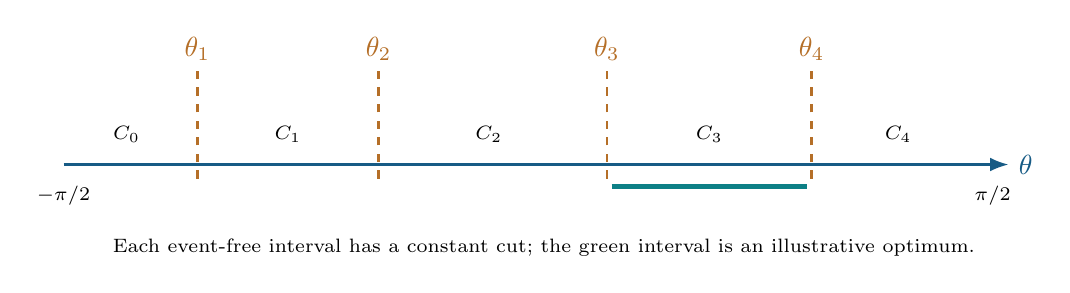
\begin{tikzpicture}[x=1cm,y=1cm]
\draw[-{Latex},thick,methodblue] (0,0)--(12,0) node[right] {$\theta$};
\foreach \x/\txt in {1.7/{\theta_1},4.0/{\theta_2},6.9/{\theta_3},9.5/{\theta_4}} {
 \draw[methodorange,dashed,thick] (\x,-0.18)--(\x,1.2);
 \node[above,methodorange] at (\x,1.2) {$\txt$};
}
\node at (.8,.38) {\scriptsize $C_0$};
\node at (2.85,.38) {\scriptsize $C_1$};
\node at (5.4,.38) {\scriptsize $C_2$};
\node at (8.2,.38) {\scriptsize $C_3$};
\node at (10.6,.38) {\scriptsize $C_4$};
\draw[ultra thick,methodteal] (6.96,-.28)--(9.44,-.28);
\node[below] at (.0,-.15) {\scriptsize $-\pi/2$};
\node[below] at (11.8,-.15) {\scriptsize $\pi/2$};
\node[align=center,font=\scriptsize] at (6.1,-1.05)
 {Each event-free interval has a constant cut; the green interval is an illustrative optimum.};
\end{tikzpicture}

\caption{A selected rotation arc is partitioned into constant-cut regions by finitely many vertex-crossing angles. Schematic illustration, not experimental measurements.}
\label{fig:events}
\end{figure}

\subsection{Actual tangent selection and search budget}
The full Experiment025 protocol attempts 250 arcs per starting normal. In \sourcecode{src/maxkcut/eva_direct_rounding.py}, proposals alternate cyclically:
\begin{enumerate}
\item \textbf{Random}: choose Gaussian $z$ and normalize $(I-rr^\top)z$.
\item \textbf{Gain-labelled}: compute $g_i=s_i(Ws)_i$, select vertices with $g_i<-10^{-9}$, and form a weighted sum of their EVA vectors, projected into $r^\perp$. The \emph{actual code selects negative-gain flips}, despite a historical comment about improving moves; a negative $g_i$ is harmful as a standalone flip.
\item \textbf{Boundary-labelled}: pick up to 96 vertices having smallest $|g_i|$, combine their vectors with random signs and project into $r^\perp$. This is \emph{not} a smallest-angular-margin rule.
\end{enumerate}
Degenerate proposals fall back to random tangents. The selected arc's best realized score replaces the incumbent only after a strict improvement. All attempted scores and modes are journaled.

\begin{algorithm}[tb]
\caption{Hyperplane Sweep: one matched GW start}\label{alg:hp}
\begin{algorithmic}[1]
\Require Graph $G$, fixed $Y$, GW normal $r_0$, $T=250$
\State $r\gets r_0$; $C\gets\cut(s(r))$
\For{$t=1,\ldots,T$}
 \State Choose the cyclic mode random/gain/boundary
 \State Generate and validate a tangent $u\perp r$
 \State $(\hat r,\hat s,\hat C)\gets\mathrm{ExactArcSweep}(G,Y,r,u)$
 \State Verify the original signed cut of $\hat s$
 \If{$\hat C>C$}
   \State $(r,C)\gets(\hat r,\hat C)$
 \EndIf
 \State Journal the attempt and accepted incumbent
\EndFor
\State \Return $r,s(r),C$
\end{algorithmic}
\end{algorithm}

\subsection{Empirical finding and limits}
The provisional Experiment025 aggregate reports mean graphwise best-of-16 gain $0.317618\%$ over refined GW, 95\% graph bootstrap interval $[0.225150,0.419601]\%$, and 59 wins, 7 ties, 5 losses among 71 graphs. Mean absolute gain is 14.08 signed cut units. Its mean relative advantage over \texttt{control-paired} is 0.045740 percentage points; a Wilcoxon graph-level signed-rank comparison of absolute cut differences reports $p=0.226$. These are different estimands. The measured performance belongs to Sweep \emph{plus} Flip/KL/ILS, not to raw hyperplane rotation alone, and the full Experiment025 source partitions still need independent off-VM auditing.

\section{Method 2: Angular Gain Greedy}\label{sec:gain}
\subsection{The meaning of the name}
The method named \sourcecode{angular-gain-greedy} combines the graph's signed single-vertex flip incentive with geometric proximity to a hyperplane crossing. Crucially, it \emph{does not directly flip vertices}. It ranks geometric tangent proposals, executes an exact signed-score sweep along each proposed arc, and accepts the best verified improvement.

Given the current unit normal $r$ and $s_i=1-2\1[y_i^\top r>0]$, the signed flip gain is $g_i=s_i(Ws)_i$ from \eqref{eq:flip}. The shortest angular distance from $r$ to the constraint $y_i^\top r=0$ is
\begin{equation}\label{eq:margin}
\delta_i=\arcsin\!\left(\frac{|y_i^\top r|}{\|y_i\|_2\|r\|_2}\right).
\end{equation}
The implemented ranking is
\begin{equation}\label{eq:priority}
q_i=\frac{\max(0,g_i)}{\delta_i+10^{-3}}.
\end{equation}
Vertices are sorted by decreasing $q_i$, then by increasing $\delta_i$, then by index. If every gain is nonpositive, small margins take precedence. The stabilizer $10^{-3}$ prevents ranking instability near a zero margin.

\subsection{Constructing a candidate tangent}
Set $a_i=y_i^\top r$, $v_i=y_i-a_ir$ and
\begin{equation}\label{eq:targettangent}
u_i=-\frac{\sigma(a_i)v_i}{\|v_i\|_2},\quad
\sigma(a)=\begin{cases}+1,&a\ge0,\\-1,&a<0.\end{cases}
\end{equation}
This is the implemented projected target direction in the tangent space $r^\perp$; degenerate projected vectors are skipped. The candidate labels are \emph{not} assigned by toggling $s_i$. Instead, \sourcecode{optimize_semicircle} tests the full continuum of event intervals along $r(\theta)$ from \eqref{eq:arc}. Multiple vertices can cross on that arc.

\subsection{Outer greedy loop}
For every round, calculate all signed gains and angular margins; form up to $K=8$ valid tangents from the highest-ranked vertices; evaluate each with the exact arc kernel and independently rescore its binary cut; select only the largest strict improvement. Stop at the first round with no improvement or after $L=32$ rounds. Thus no more than 256 arcs are considered per seed, although early stopping normally reduces the count. The full source logs every proposed vertex, signed gain, angle, realized cut and accepted normal.

\begin{algorithm}[tb]
\caption{Angular Gain Greedy}\label{alg:gain}
\begin{algorithmic}[1]
\Require $G$, frozen $Y$, GW normal $r$, $K=8$, $L=32$
\State $C\gets\cut(s(r))$
\For{$t=1,\ldots,L$}
 \State Compute $g_i=s_i(Ws)_i$ and $\delta_i$; rank vertices by \eqref{eq:priority}
 \State $(r_{\rm next},C_{\rm next})\gets(r,C)$
 \For{up to $K$ nondegenerate ranked targets $i$}
  \State Build tangent $u_i$ from \eqref{eq:targettangent}
  \State $(\hat r,\hat s,\hat C)\gets\mathrm{ExactArcSweep}(G,Y,r,u_i)$
  \State Rescore $\hat s$ and journal every attempted cut
  \If{$\hat C>C_{\rm next}$}
   \State $(r_{\rm next},C_{\rm next})\gets(\hat r,\hat C)$
  \EndIf
 \EndFor
 \If{$C_{\rm next}\le C$}\State \textbf{break}\EndIf
 \State $(r,C)\gets(r_{\rm next},C_{\rm next})$; archive accepted normal
\EndFor
\State \Return realized normal, labels and signed cut
\end{algorithmic}
\end{algorithm}

\subsection{Findings}
Experiment027 independently audits 71 graphs, 16 matched starts, and this new method's four-stage journal. The mean post-refinement gain versus refined GW is $R_{\mathrm{gain}}=0.316704\%$, with graph-bootstrap interval $[0.233363,0.403293]\%$ and 61/8/2 graph wins/ties/losses. Against the \emph{historical} Hyperplane Sweep, the best-of-16 comparisons are 30/10/31; average signed-cut difference $-0.310$ units. Across \emph{matched individual seeds}, raw angular gain minus raw Sweep averages $-17.031$ units, while the final best-stage delta averages $-0.971$. These different estimands show that later Flip/KL/ILS can mask substantial raw rounding differences. The source records 65,488 attempted arcs across 1,136 starts (not 256 arcs executed per start).

\section{Method 3: Angular Margin Greedy}\label{sec:margin}
\subsection{What changes relative to Angular Gain?}
The geometric state, exact arc sweep, $K=8$ candidate budget, $L=32$ outer-round cap and strict acceptance logic are \emph{identical} to the previous section. Only the \emph{target-ordering rule} changes. The name \sourcecode{angular-margin-greedy} means that vertices closest to the moving hyperplane boundary have first priority, without using $g_i$ to rank them. Compute
\[
\delta_i=\arcsin\left(\frac{|y_i^\top r|}{\|y_i\|_2}\right)
\]
for unit $r$, and sort by increasing $\delta_i$, breaking ties by vertex index. Use exactly the projected tangent \eqref{eq:targettangent} for each candidate vertex and call the same exact, original-signed \sourcecode{optimize_semicircle} kernel.

\subsection{Why this is a meaningful ablation}
The margin $\delta_i$ quantifies how far the current normal must rotate before vertex $i$ can lie exactly on the separating boundary. For fixed $r$, smaller $\delta_i$ means a crossing is geometrically accessible by a shorter great-circle motion. The method tests whether such proximity is itself a useful candidate signal. It does \emph{not} assume that flipping the closest vertex improves the signed objective. Every candidate arc is rescored on the original weighted graph; even a nearest boundary is rejected if it does not lead to a strict gain.

\begin{algorithm}[tb]
\caption{Angular Margin Greedy}\label{alg:margin}
\begin{algorithmic}[1]
\Require $G,Y,r_0$, $K=8$, $L=32$
\State $r\gets r_0$; $C\gets\cut(s(r))$
\For{$t=1,\ldots,L$}
 \State Compute all $\delta_i$ and sort vertices by $(\delta_i,i)$
 \State Initialize the next best result to current $(r,C)$
 \For{the first $K$ nondegenerate target tangents $u_i$}
  \State Exactly sweep all original-signed crossing events along $(r,u_i)$
  \State Keep the best independently verified strict improvement
 \EndFor
 \If{no tested arc improves $C$} \State \textbf{break}\EndIf
 \State Accept one best arc; update the normal and archive the event
\EndFor
\State \Return the final feasible hyperplane and raw cut
\end{algorithmic}
\end{algorithm}

\subsection{Analytical observations}
Unlike a differentiable optimization algorithm, the landscape of $F(r)$ is piecewise constant. A conventional gradient is zero almost everywhere and cannot identify which crossing produces a positive cut change. The margin ranking controls the \emph{geometric distance} to an event but omits the \emph{graph cost} of that event. In contrast, Gain ranks by both $g_i$ and $\delta_i$. Their difference is an interpretable source of testable hypotheses, not proof that either dominates on every graph.

\subsection{Measured performance}
The independently audited 71-graph post-refinement mean gain is $0.302682\%$ versus refined GW (95\% graph bootstrap $[0.213226,0.400243]\%$), with 56/9/6 graph wins/ties/losses. It beats/ties/loses against the historical Hyperplane Sweep on 29/14/28 graphs; the average best-of-16 cut difference is $-1.000$ original signed unit. The matched-seed mean raw difference to Sweep is $-16.807$ units and final-stage best difference is $-1.463$. The archive reports 62,888 attempted sweeps across 1,136 starts. These values describe original signed cuts, not geometric distances or approximation guarantees.

\section{Method 4: Angular Pair Greedy}\label{sec:pair}
\subsection{Why target a pair?}
The name \sourcecode{angular-pair-greedy} refers to a \emph{pair of desired hyperplane-crossing constraints}, not a direct two-vertex combinatorial flip. At a current unit normal $r$, a single vertex $i$ is on the separating boundary when $y_i^\top r=0$. For two vertices, the simultaneous linear constraints are
\begin{equation}\label{eq:pairconstraints}
y_i^\top r_{\rm target}=0,\qquad
y_j^\top r_{\rm target}=0.
\end{equation}
This asks for a normal in the common orthogonal complement of $y_i$ and $y_j$, if it is nonempty.

\subsection{Actual pair selection and tangent geometry}
First calculate $g_i=s_i(Ws)_i$, $\delta_i$ and $q_i$ as in Angular Gain. Rank vertices by decreasing $q_i$ and increasing $\delta_i$. Make a pool from the first $\min(n,\max(2K,8))$ vertices ($K=8$ in the full protocol). Enumerate pairs in that pool, sorting them by decreasing $q_i+q_j$, then increasing $\delta_i+\delta_j$, then lexicographic vertex indices. Attempt the first $K$ valid pair tangents.

For a selected pair, put $A=[y_i\ \ y_j]\in\R^{p\times2}$. If $A$ is rank deficient, the current implementation skips the pair. Otherwise, project the current normal into the orthogonal complement:
\begin{equation}\label{eq:pairproject}
z=r-A(A^\top A)^+A^\top r,\quad
t=\frac{z}{\|z\|_2},\quad
u=\frac{t-(t^\top r)r}{\|t-(t^\top r)r\|_2}.
\end{equation}
The implementation orients $t$ so that $t^\top r\ge0$, and skips numerically invalid or vanishing projections. Here $(\cdot)^+$ is a pseudoinverse. The construction aims toward a normal satisfying \eqref{eq:pairconstraints}, but the subsequent \emph{exact semicircle sweep} may choose a better interval \emph{before or beyond} those crossings.

\begin{algorithm}[tb]
\caption{Angular Pair Greedy}\label{alg:pair}
\begin{algorithmic}[1]
\Require $G,Y,r_0$, $K=8$, $L=32$
\State $r\gets r_0$; $C\gets\cut(s(r))$
\For{$t=1,\ldots,L$}
 \State Compute $q_i,\delta_i$ and select the top-$\max(2K,8)$ vertex pool
 \State Rank pairs by $-(q_i+q_j)$, $\delta_i+\delta_j$, then indices
 \State Initialize next best to $(r,C)$
 \For{up to $K$ valid ranked pairs $(i,j)$}
  \State Project $r$ using \eqref{eq:pairproject} to obtain $u$
  \State Exactly sweep the arc $(r,u)$; independently rescore all candidates
  \State Retain the strongest strict candidate and journal its pair
 \EndFor
 \If{no improvement} \State \textbf{break}\EndIf
 \State Accept the best verified new normal, and journal its partition
\EndFor
\end{algorithmic}
\end{algorithm}

\subsection{Geometry and conditional limitations}
Targeting two boundaries introduces interaction information at the \emph{proposal} level but does not exactly solve a best double-flip graph problem. Pair selection does not enforce both intended vertices to cross at the chosen arc maximizer, nor does it enumerate all $\binom n2$ pairs. Its additional rank condition and pseudoinverse cost can discard seemingly attractive targets. Every accepted partition is still a valid homogeneous hyperplane cut of the fixed $Y$.

\subsection{Measured performance}
The independently audited mean best-of-16 gain is $0.281426\%$ versus refined GW, with graph-bootstrap interval $[0.198963,0.367844]\%$ and 56/7/8 graph wins/ties/losses. Against the historical Hyperplane Sweep, it wins/ties/loses 28/9/34 graphs and has mean absolute best-of-16 signed-cut difference $-1.085$ units. The mean matched-seed raw difference is $-16.145$ units; the corresponding mean final best-stage difference is $-2.160$. Across 1,136 seeds the journal records 65,320 attempted great-semicircle paths. The fact that this pair heuristic does not beat the simpler single-target guidance globally is an observed negative result worth preserving.

\section{Method 5: Paired Spherical K-Means Control}\label{sec:paired}
\subsection{The paired two-center initialization}
The exact method name is \sourcecode{control-paired}; the term \emph{paired} means that the two \emph{centers} are antipodal. It is the historical K-MeansNM rule, applied to the \emph{same GW normal} shared by the other protocols:
\begin{equation}\label{eq:pairedinit}
c_0^{(0)}=-r_0,\qquad c_1^{(0)}=r_0.
\end{equation}
This pairing is distinct from the statistical matching of 16 normal vectors across experiments. The method is an adaptive spherical clustering initializer, not a modified EVA factor.

\subsection{Lloyd updates}
For unit-norm EVA vectors $y_i$, the assignment stage maximizes cosine similarity:
\begin{equation}\label{eq:lloydassignment}
\ell_i^{(t)}=\argmax_{a\in\{0,1\}}y_i^\top c_a^{(t)}.
\end{equation}
Let $V_a^{(t)}=\{i:\ell_i^{(t)}=a\}$. A nonempty cluster updates its center to the normalized spherical mean:
\begin{equation}\label{eq:lloydcenters}
c_a^{(t+1)}
=\frac{\sum_{i\in V_a^{(t)}}y_i}
{\left\|\sum_{i\in V_a^{(t)}}y_i\right\|_2}.
\end{equation}
Degenerate or empty-center cases use a seeded fallback. At most 100 Lloyd iterations run in the full protocol, or fewer if the labels stabilize. The first assignment has exactly the initial GW split (apart from zero-projection tie conventions), because the difference of the initial similarities is $2y_i^\top r_0$. Later centers may cease to be antipodal, but their binary nearest-center decision is still induced by the homogeneous normal $c_1-c_0$.

\subsection{Original-cut retention versus clustering inertia}
Spherical Lloyd updates optimize a geometric association measure; they do not directly maximize weighted signed Max-Cut. The implementation separately evaluates the \emph{original signed graph} at every Lloyd assignment and saves the best cut found along the trajectory, including the initial GW split. In particular, the retained raw best cannot be worse than its own initial GW cut, even though an individual unretained Lloyd step may be worse.

\begin{algorithm}[tb]
\caption{Paired spherical K-MeansNM}\label{alg:paired}
\begin{algorithmic}[1]
\Require $G$, frozen $Y$, shared normal $r_0$
\State Initialize $c_0=-r_0,c_1=r_0$ and retain original GW labels
\For{$t=1,\ldots,100$}
 \State Set labels by \eqref{eq:lloydassignment}
 \State Score the original signed cut and update best-so-far
 \If{assignments have converged}\State\textbf{break}\EndIf
 \State Update nonempty cluster centers by \eqref{eq:lloydcenters}
\EndFor
\State \Return best observed binary partition and original signed score
\end{algorithmic}
\end{algorithm}

\subsection{Experiment025 findings}
The provisional 71-graph aggregate reports mean graphwise best-of-16 improvement $0.271877\%$ (95\% graph-bootstrap interval $[0.178158,0.372921]\%$) versus refined GW. Graphwise wins/ties/losses are 55/8/8. Hyperplane Sweep beats/ties/loses against this control on 36/10/25 graphs, but a paired graphwise Wilcoxon test on absolute signed-cut differences reports $p=0.2256$; it does not resolve the two top methods on that test. This result demonstrates the value of structured centroid search \emph{after the common refiner}, not that spherical K-Means produces a globally optimal raw cut.
\section{Method 6: Soft EM Followed by Gibbs Annealing}\label{sec:gibbs}
\subsection{One method name, two distinct algorithms}
The name \sourcecode{em-gibbs} is a \emph{soft EM-like optimization of Bernoulli membership probabilities}, followed by a temperature-annealed Gibbs sampler acting on a hard binary graph partition. The EM-like first stage is \emph{not} maximum-likelihood Gaussian mixture modeling: it optimizes a stated entropy-regularized signed-cut objective with spherical-centroid alignment.

\subsection{The soft free energy and conditional probability update}
Let $p_i\in(0,1)$ denote the probability of side 1, assuming independent Bernoulli variables for the soft expected-cut calculation. Let $c_0,c_1$ be unit spherical centers, $\kappa\ge0$ their geometric weight, and $T>0$ temperature. The implementation's free energy is
\begin{align}\label{eq:freeenergy}
\mathcal L_T(p,c_0,c_1)
={}&\sum_{\{i,j\}\in E}
 w_{ij}(p_i+p_j-2p_ip_j)\nonumber\\
&+\kappa\sum_i\bigl[(1-p_i)y_i^\top c_0+
                           p_i y_i^\top c_1\bigr]+T\sum_iH(p_i),\\
H(p)&=-p\log p-(1-p)\log(1-p).\nonumber
\end{align}
The first term is the expected original signed cut because $\Pr(\ell_i\ne\ell_j)=p_i+p_j-2p_ip_j$. Differentiating with respect to $p_i$, holding the other memberships and centroids fixed, gives
\[
\frac{\partial\mathcal L_T}{\partial p_i}
=\sum_jw_{ij}(1-2p_j)+\kappa y_i^\top(c_1-c_0)
 +T\log\frac{1-p_i}{p_i}.
\]
The conditional stationary target therefore satisfies
\begin{equation}\label{eq:softupdate}
p_i^{\rm target}=
\operatorname{sigmoid}\!\left(
\frac{[W(1-2p)]_i+\kappa\,y_i^\top(c_1-c_0)}{T}\right).
\end{equation}
The implementation performs a \emph{damped, synchronous} probability update with backtracking if free energy decreases. For fixed memberships, the geometric M-step is
\begin{equation}\label{eq:softcenters}
c_0=\frac{\sum_i(1-p_i)y_i}{\|\sum_i(1-p_i)y_i\|_2},
\qquad
c_1=\frac{\sum_i p_i y_i}{\|\sum_i p_i y_i\|_2},
\end{equation}
with a degenerate-center fallback. Temperature changes between stages, so a monotonicity statement applies within each fixed-$T$ stage only.

Experiment025 initializes $p_i=0.95$ or $0.05$ depending on the \emph{same current GW partition}, recalculates centroids, uses eight geometrically spaced temperature stages and up to 20 soft iterations per stage. This is not a historical elite warm start. The soft stage hardens with $\ell_i=\1[p_i\ge1/2]$.

\subsection{Gibbs heat-bath flips and derivation}
For a current hard spin partition $s$ and vertex gain $g_i=s_i(Ws)_i$, compare the two conditional scores that differ only at $i$. Their cut-value difference is $g_i$. At temperature $T$, the probability of choosing the opposite spin is
\begin{equation}\label{eq:gibbs}
\Pr(\mathrm{flip}\ i\mid s_{-i},T)
=\frac{\exp((\cut(s)+g_i)/T)}
{\exp(\cut(s)/T)+\exp((\cut(s)+g_i)/T)}
=\operatorname{sigmoid}(g_i/T).
\end{equation}
Positive gains are favored, but negative gains are allowed with positive probability; this is how annealing can move across poor intermediate partitions. The implemented full protocol cools from $T=12$ to $0.4$ over 150 sweeps, visits vertices in a seeded random order, and retains the best original signed hard cut. The Gibbs walker may deteriorate before finding a better candidate. Gibbs updates operate directly on labels and are not restricted to hyperplane-realizable partitions.

\begin{algorithm}[tb]
\caption{EM--Gibbs before the common postprocessor}\label{alg:gibbs}
\begin{algorithmic}[1]
\Require $G,Y$, shared GW labels, soft and Gibbs temperature schedules
\State Initialize $p_i$ at $0.95/0.05$ according to the shared GW partition
\State Initialize spherical centroids from soft memberships
\For{each of 8 soft-temperature stages}
 \For{up to 20 damped EM-like updates}
  \State Propose memberships by \eqref{eq:softupdate}; backtrack if needed
  \State Update centroids by \eqref{eq:softcenters}; audit free energy
 \EndFor
\EndFor
\State Harden memberships to a feasible original signed cut
\For{150 cooling Gibbs sweeps}
 \For{each vertex in seeded order}
  \State Calculate $g_i$ and flip with probability \eqref{eq:gibbs}
  \State Retain every improved original signed hard cut
 \EndFor
\EndFor
\State \Return best hard partition (not necessarily a hyperplane cut)
\end{algorithmic}
\end{algorithm}

\subsection{Empirical finding and limits}
The provisional Experiment025 aggregate gives mean graphwise best-of-16 gain $0.270688\%$ over refined GW, with 95\% bootstrap interval $[0.195602,0.352190]\%$ and 59/9/3 graph wins/ties/losses. Hyperplane Sweep wins/ties/loses against EM--Gibbs on 36/9/26 graphs, with a two-sided signed-rank $p=0.1633$ on absolute cut differences. This full-protocol competitiveness does not imply that raw Gibbs partitions are linearly separable. Moreover, the code uses stochastic label search, so the method should not be counted as a pure geometric hyperplane rounder in a later no-KL/no-ILS experiment.

\section{Method 7: Cut-aware Spherical K-Means}\label{sec:cutaware}
\subsection{How the name differs from ordinary K-Means}
The method \sourcecode{cutaware-kmeans} begins with the GW-paired spherical Lloyd trajectory, but it scores the \emph{original signed graph} when selecting directions. It then tests perturbed, centroid-based and gain-weighted directions. For each such direction, it finds the \emph{exact best affine threshold} conditional on that direction. Thus the method searches both directions and offsets, but is only exact in one dimension at a time.

\subsection{An exact threshold conditional on one direction}
For a fixed unit direction $d$, let $z_i=y_i^\top d$. With offset $b$, choose $\ell_i(b)=\1[z_i>b]$. The binary partition changes only as $b$ crosses one of the sorted projection values $z_i$; tied projections must move together. The best signed cut for this fixed direction is
\begin{equation}\label{eq:threshold}
\max_{b\in\R}\cut\bigl(1-2\1[Yd>b]\bigr).
\end{equation}
Sorting the $z_i$ and sweeping all attainable event groups with the exact gain \eqref{eq:flip} costs $O(np+n\log n+m)$, including the projection. This is \emph{not} an exact global optimization over all $d$; the best threshold can also yield unbalanced sides, since no balance constraint is imposed.

\subsection{The six implemented proposal actions}
The full Experiment025 protocol starts spherical Lloyd with centers $(-r_0,r_0)$, at most 100 iterations, and considers every center-difference direction $d=c_1-c_0$. It additionally attempts 96 direction trials by cycling through six actions:
\begin{enumerate}
\item The first four actions add Gaussian noise to an incumbent good direction or a fresh random normal. Experiment025's paired implementation uses perturbation scales $0.05$ and $0.20$.
\item The fifth action computes the two spherical centroids of the \emph{current winning partition} and proposes their normalized difference.
\item The sixth constructs a graph-aware direction from the incumbent labels and signed gains:
\begin{equation}\label{eq:proxy}
q_i=\frac{1}{1+|g_i|},\qquad
d\propto\sum_i(2\ell_i-1)q_i y_i.
\end{equation}
\end{enumerate}
Note the important implementation nuance in \eqref{eq:proxy}: \emph{small absolute flip gains receive higher weights}. This proposal is not the mathematical derivative of the discontinuous original cut with respect to $d$. Each direction is normalized, subjected to exact threshold search, and independently scored against the actual signed graph. The incumbent retains the highest scored candidate, including the original K-MeansNM trajectory.

\begin{algorithm}[tb]
\caption{Cut-aware spherical K-Means and threshold search}\label{alg:cutaware}
\begin{algorithmic}[1]
\Require $G,Y$, common GW normal $r_0$, 100 Lloyd iterations, 96 trials
\State Initialize two centers at $(-r_0,r_0)$
\For{each Lloyd iteration}
 \State Obtain the current spherical partition and its centroid difference $d$
 \State Exactly optimize the offset of $d$ using \eqref{eq:threshold}
 \State Keep the best verified signed cut; update spherical centroids
\EndFor
\For{each of 96 direction trials}
 \State Choose Gaussian perturbation, centroid-difference or \eqref{eq:proxy}
 \State Normalize $d$, solve the exact fixed-$d$ threshold sweep
 \State Independently rescore and retain the best original signed cut
\EndFor
\State \Return best binary partition, direction and offset diagnostics
\end{algorithmic}
\end{algorithm}

\subsection{Geometric interpretation}
A linear separator with threshold $b$ has labels $\sign(y_i^\top d-b)$. Since
$\sign(y_i^\top d-b)=\sign((y_i,1)^\top(d,-b))$, affine separators in $\R^p$ are origin-passing separators in $\R^{p+1}$ after augmentation. This is merely a geometric reformulation of the rounding family; it does not recompute the SDP or automatically preserve a GW approximation guarantee. Cut-aware K-Means is therefore a natural candidate for \emph{raw-only} affine-hyperplane experiments, unlike Gibbs or direct vertex flips.

\subsection{Empirical finding}
Experiment025's provisional mean graphwise post-refinement gain is $0.266807\%$ over refined GW, with 95\% graph-bootstrap interval $[0.177533,0.363149]\%$ and 56/5/10 graph wins/ties/losses. Against Cut-aware K-Means, Hyperplane Sweep wins/ties/loses 41/7/23 graphs; its mean relative advantage is $0.050811$ percentage points, while the signed-rank $p$-value on absolute cut differences is $0.110$. Neither comparison justifies calling the threshold optimizer a global solution to Max-Cut.

\section{Integrated empirical findings}\label{sec:results}
\subsection{The complete seven-method ordering}
\Cref{tab:seven} reproduces the seven highest relative best-of-16 scores among the 18 historical protocols plus the three independently audited new angular variants. A ranked list is useful for exposition but is \emph{not} a significance ordering. In particular, the top two values differ by only $0.000914$ percentage points; such a small descriptive difference must not be interpreted as proof of superiority.
\begin{table}[tb]
\centering\small
\caption{The selected seven by equal-graph mean post-refinement best-of-16 improvement over the \emph{refined} GW-RR control. Confidence intervals bootstrap graphs (E025: 30,000 draws; E027: 2,000). W/T/L is versus \emph{refined GW}. E025 is still provisionally supported by its 1,278-row aggregate; E027 has an independent five-method archive audit.}\label{tab:seven}
\begin{tabular}{@{}rlcccc@{}}
\toprule
Rank & Method & Gain (\%) & 95\% graph interval (\%) & W/T/L vs GW & Source\\
\midrule
1 & Hyperplane Sweep      & 0.317618 & [0.225150, 0.419601] & 59/7/5 & E025\\
2 & Angular Gain Greedy   & 0.316704 & [0.233363, 0.403293] & 61/8/2 & E027\\
3 & Angular Margin Greedy & 0.302682 & [0.213226, 0.400243] & 56/9/6 & E027\\
4 & Angular Pair Greedy   & 0.281426 & [0.198963, 0.367844] & 56/7/8 & E027\\
5 & Paired K-Means Control& 0.271877 & [0.178158, 0.372921] & 55/8/8 & E025\\
6 & EM--Gibbs             & 0.270688 & [0.195602, 0.352190] & 59/9/3 & E025\\
7 & Cut-aware K-Means     & 0.266807 & [0.177533, 0.363149] & 56/5/10 & E025\\
\bottomrule
\end{tabular}
\end{table}

\begin{figure}[tb]
\centering
\begin{tikzpicture}[x=10cm,y=0.65cm]
\draw[->,thin] (0,0.2)--(0.49,0.2) node[right,font=\scriptsize]{mean gain (\%)};
\foreach \t in {0,0.1,0.2,0.3,0.4} {
  \draw[gray!30] (\t,0.35)--(\t,7.5);
  \node[font=\scriptsize,anchor=north] at (\t,0.18) {\t};
}
\foreach \y/\name/\v/\lo/\hi/\col in {
7/{Hyperplane Sweep}/0.317618/0.225150/0.419601/methodblue,
6/{Angular Gain}/0.316704/0.233363/0.403293/methodteal,
5/{Angular Margin}/0.302682/0.213226/0.400243/methodteal,
4/{Angular Pair}/0.281426/0.198963/0.367844/methodteal,
3/{Paired K-Means}/0.271877/0.178158/0.372921/methodblue,
2/{EM--Gibbs}/0.270688/0.195602/0.352190/methodblue,
1/{Cut-aware K-Means}/0.266807/0.177533/0.363149/methodblue
} {
 \node[font=\scriptsize,anchor=east] at (-0.012,\y) {\name};
 \fill[\col!40] (0,\y-0.21) rectangle (\v,\y+0.21);
 \draw[\col,line width=.7pt] (\lo,\y)--(\hi,\y);
 \draw[\col,line width=.7pt] (\lo,\y-.11)--(\lo,\y+.11);
 \draw[\col,line width=.7pt] (\hi,\y-.11)--(\hi,\y+.11);
 \node[font=\tiny,anchor=west] at (\v+0.008,\y+0.22) {\pgfmathprintnumber[fixed,precision=3]{\v}};
}
\node[font=\scriptsize,anchor=west,text=methodblue] at (0,7.92) {E025 provisional};
\node[font=\scriptsize,anchor=west,text=methodteal] at (0.23,7.92) {E027 audited};
\end{tikzpicture}

\caption{Source-reported seven-method mean graphwise gains and 95\% bootstrap intervals from the two historical audits. A comparison of marginal intervals is \emph{not} a paired test of between-method differences; the two colors distinguish source/audit status.}
\label{fig:ranking}
\end{figure}

\subsection{Direct comparison with Hyperplane Sweep}
For Experiment027, matched comparisons against the historical HP comparator are available at \emph{both} raw and refined stages. Best-of-16 graph counts versus HP are Gain 30/10/31, Margin 29/14/28 and Pair 28/9/34, with respective mean best-of-16 cut differences $-0.310$, $-1.000$ and $-1.085$ units. None has established a consistent single-method advantage. Their 95\% \emph{exploratory} graph-bootstrap intervals for mean absolute differences against HP overlap zero; these were post-publication descriptive computations, not a prospective multiple-comparison test.

For E025's three selected non-HP methods, the historical aggregate provides the opposite orientation of W/T/L (HP against each):
\[
\begin{array}{lll}
\text{HP vs paired:}&36/10/25,&
\text{HP vs EM--Gibbs:}\ 36/9/26,\\
\text{HP vs cut-aware:}&41/7/23.&&
\end{array}
\]
The E025 graphwise Wilcoxon signed-rank $p$-values for these \emph{absolute cut differences} are respectively $0.2256$, $0.1633$ and $0.1097$. No multiplicity-adjusted cross-study head-to-head superiority has been established. Bootstrap intervals for mean \emph{relative gain} and Wilcoxon tests for \emph{absolute signed differences} have different targets and can legitimately disagree.

\subsection{Why the raw endpoint changes the interpretation}
The audited E027 per-seed comparison provides the following paired means over 71 graphs times 16 shared start indices:
\begin{table}[tb]
\centering\small
\caption{New angular method minus historical HP in signed cut \emph{units}. Means use all 1,136 matched graph--seed pairs per new method; they are not best-of-16 maxima.}\label{tab:raw}
\begin{tabular}{@{}lrrr@{}}
\toprule
Method & Raw round cut minus HP & Final best-stage minus HP & Best-of-16 graph difference\\
\midrule
Angular Gain Greedy   & $-17.031$ & $-0.971$ & $-0.310$\\
Angular Margin Greedy & $-16.807$ & $-1.463$ & $-1.000$\\
Angular Pair Greedy   & $-16.145$ & $-2.160$ & $-1.085$\\
\bottomrule
\end{tabular}
\end{table}
The raw gap is an order of magnitude larger than the after-refinement gap. This is a \emph{negative result for the interpretation of raw angular search} under the recorded starting budget, even though all three full protocols outperform refined GW on average. The multiple maxima and mean-of-seeds are not algebraically interchangeable: $\max_t(C_a-C_b)$ and $\max_t C_a-\max_t C_b$ are different quantities.

\begin{figure}[tb]
\centering
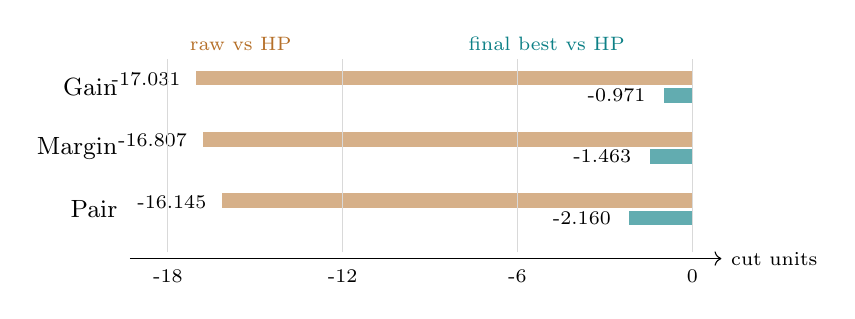
\begin{tikzpicture}[x=0.37cm,y=.78cm]
\foreach \y/\name/\raw/\final in {
3/{Gain}/-17.031/-0.971,
2/{Margin}/-16.807/-1.463,
1/{Pair}/-16.145/-2.160
} {
\node[anchor=east,font=\small] at (-19.4,\y) {\name};
\fill[methodorange!55] (\raw,\y+0.02) rectangle (0,\y+0.26);
\fill[methodteal!65] (\final,\y-0.26) rectangle (0,\y-0.02);
\node[font=\scriptsize,anchor=east] at (\raw-.2,\y+.12) {\raw};
\node[font=\scriptsize,anchor=east] at (\final-.3,\y-.14) {\final};
}
\draw[->,thin] (-19.3,.2)--(1,.2) node[right,font=\scriptsize]{cut units};
\foreach \x in {-18,-12,-6,0} {
\draw[gray!30] (\x,.3)--(\x,3.45);
\node[anchor=north,font=\scriptsize] at (\x,.18) {\x};
}
\node[font=\scriptsize,text=methodorange] at (-15.5,3.7) {raw vs HP};
\node[font=\scriptsize,text=methodteal] at (-5.0,3.7) {final best vs HP};
\end{tikzpicture}

\caption{Mean paired-seed raw and final-best signed cut differences from historical Hyperplane Sweep (Experiment027). The common refiner greatly reduces the initial raw disadvantage; these are not graphwise best-of-16 maxima.}
\label{fig:rawgap}
\end{figure}

\subsection{Recorded work is not equal work}
The three E027 angular methods evaluated 65,488, 62,888 and 65,320 arcs respectively over their 1,136 starts; the original HP protocol nominally budgets up to 250 attempts per start. Reported mean per-seed wall times are approximately GW $0.937$ s, HP $2.487$ s, Gain $0.996$ s, Margin $1.057$ s and Pair $0.983$ s. These descriptive archived times are not a controlled equal-hardware benchmark: E025's aggregate wall-time field is the last invocation, not total 16-seed work, and method-specific preprocessing and attempted events differ substantially. We therefore do not claim a causal speedup or a demonstrated equal-budget quality improvement.

The in-sample portfolio taking the best of the three angular results \emph{after running all three} beats HP on 42 graphs, ties on 13 and loses on 16, with mean best-of-16 signed-cut difference $+2.761$ units. This spends a larger search budget and uses an ex post oracle choice; it is not a deployable equal-cost algorithm.

\subsection{Graph families and limitations}
The Experiment025 Hyperplane Sweep mean relative gain over GW is reported as $+0.375\%$ on the 30 random graphs, $+0.411\%$ on 24 planar-family graphs and $+0.084\%$ on 17 toroidal graphs. Within 35 positive-weight graphs it is $+0.163\%$ and within 36 signed-weight graphs $+0.468\%$. Graph families and edge signs are not independently randomized and can be confounded. No causal structure-dependent method recommendation follows. The old archive status, source differences and post-hoc selection limit inferential scope.

All published values in this section are transcribed from the committed E025 method-ranking and head-to-head CSVs and the E027 independently audited comparison CSV/JSON. The manuscript's \sourcecode{data/top_seven.csv} is a \emph{derived presentation table}, not a replacement for those primary files. The accompanying checker validates both sources at each build.

\section{Discussion, rival explanations, and research priorities}\label{sec:discussion}
\subsection{What is common and what is truly different?}
Six of the seven methods manipulate a hyperplane or spherical geometry at some stage, but they search quite different families of raw feasible cuts. Hyperplane Sweep and the three Angular Greedy variants accept normals of \emph{homogeneous} origin hyperplanes; Cut-aware K-Means considers \emph{affine} offsets; Paired Spherical K-Means updates two centroids whose difference determines a homogeneous binary separator; EM--Gibbs probabilistically flips binary labels, with no hyperplane-separability guarantee. The shared postprocessor eliminates any guarantee of hyperplane separability from the final solution, regardless of its initializer.

All seven use the \emph{same saved embedding}, but their algorithm-specific work differs. The best-of-16 quality ranking is neither a list of seven approximation-ratio improvements nor a proof that their mean differences are statistically distinguishable. Exactness of the \emph{one-dimensional event scan} is conditional on the chosen path, numerical tolerances and event grouping; finite greedy proposal lists cannot globally solve Max-Cut.

\subsection{Thesis, antithesis, synthesis}
\paragraph{Thesis.} Geometric information in a fixed SDP-derived factor is useful: the historical full refined protocols each improve over a similarly refined GW control on a majority of graphs. Hyperplane Sweep's position, and the competitiveness of angular and spherical alternatives, motivate a deeper theory of rounding landscapes.

\paragraph{Antithesis.} The historical ranking is partly provisional, post-hoc method selection favors candidates tested on the same graphs, unequal candidate budgets prevent a pure efficiency comparison, and E027's raw angular results are \emph{worse} than HP on average per matched seed. Strong downstream KL/ILS may obscure weak rounding initializers; EM--Gibbs is not even a hyperplane-only method.

\paragraph{Synthesis.} Analyze the \emph{raw original signed cut} $F(r,b)=\cut(\sign(Yr-b\mathbf{1}))$ as a function of an oriented and translated hyperplane, independent of all unrestricted label-space postprocessing. The score is piecewise constant in the normal/offset parameters. Crossing events are determined by geometry, while jumps in the score depend on the signed adjacency through \eqref{eq:flip}. An affine plane can be viewed as a homogeneous separator in the augmented embedding $[Y\mid\mathbf{1}]$. Yet if $\operatorname{rank}(Y)=n$, every binary spin vector is representable by a homogeneous normal, so unrestricted best-hyperplane search may be as difficult as Max-Cut itself. The distinction between \emph{conditional path exactness} and \emph{global search} remains fundamental.

\subsection{Recommended future experiments}
A prospective follow-up should freeze the original 71 graph inputs and the saved EVA factors and start from the identical 16 GW normals. Pre-register arms for random GW, exact threshold translation, exact origin rotation, alternating rotate/translate updates, and augmented-space joint search. Require \emph{no Flip, KL, ILS, Tabu or other direct label correction} in the primary comparison. Record complete per-iteration accepted normals, offsets, events, raw partitions, verified cut weights, geometric margins, signed gains, factor and graph SHA values, and CPU/event counts. Compare matched computational budgets, not merely matched numbers of GW starts, and validate on held-out graph families. A low-rank truncation ablation would probe how the expressible hyperplane partitions change with factor rank. Do not interpret this plan as completed Experiment028 results.

\section{Conclusion}
The seven leading recorded protocols can be derived from a small number of principles: exact hyperplane event sweeps, heuristic tangent ranking, spherical centroid updates, entropy-regularized soft membership search, Gibbs annealing, and exact affine threshold sweeps. All seven show positive average \emph{post-refinement} best-of-16 gains over refined GW in the saved studies, but no unique statistically established cross-method champion or compute-normalized superiority follows. The strongest open scientific question is whether optimizing the rounding geometry alone yields a meaningful improvement \emph{before} unrestricted label search.


\appendix
\section{Additional derivations and invariants}\label{app:proofs}
\subsection{Why the affine threshold is exact for a fixed normal}
For any fixed $d$, define $z_i=y_i^\top d$ and the cut assignment $\ell_i(b)=\1[z_i>b]$. There are at most $n+1$ open intervals between distinct projections, including the two outer intervals. On each interval, $\ell_i(b)$ and $\cut$ are constant. By sorting $z_i$ and applying the signed flip gain \eqref{eq:flip} to each tied crossing group, the algorithm evaluates every attainable cut. The maximum of those cut scores is therefore exact \emph{conditional on $d$}. As the direction changes, the order of projected vertices can also change; this is why one sorting operation does not solve the full affine problem.

\subsection{Pair projection and its rank condition}
For rank-two $A=[y_i\ y_j]$ with $p\ge3$, the matrix $P_{A^\perp}=I-A(A^\top A)^+A^\top$ is the orthogonal projector onto the common null space of $y_i^\top$ and $y_j^\top$. For nonzero $z=P_{A^\perp}r$, $t=z/\|z\|$ satisfies $A^\top t=0$. The tangent $u\propto t-(r^\top t)r$ satisfies $r^\top u=0$, giving a candidate great circle. However, $\theta$ is then chosen by maximizing the \emph{entire original signed cut on that arc}; it need not make both selected vertices switch sides.

\subsection{Strict-incumbent retention}
Let $C_t$ be the independently verified current incumbent after the $t$th proposal round and $\widehat C_t$ the best realized candidate of that round. Setting $C_{t+1}=\max(C_t,\widehat C_t)$ gives $C_{t+1}\ge C_t$. This guarantees a nondecreasing \emph{saved incumbent}, not nondecreasing Lloyd assignments, Gibbs walker states or current ILS states. There are finitely many binary partitions, but a finite proposal budget does not imply global or locally exhaustive optimality.

\subsection{Original signed versus nonnegative-weight interpretations}
For an edge with $w_{ij}<0$, separating its endpoints \emph{reduces} the objective, and a graph with both signs can favor leaving certain negative edges uncut. A probabilistic or directional proposal justified only for a nonnegative graph must still be independently scored on the signed original edges. In particular, approximation-factor statements for the classical GW nonnegative-weight objective are not automatically inherited by any of these finite heuristic perturbations or the approximate EVA factor. This distinction is both mathematical and an implementation-level archive invariant.

\subsection{The empirical maximum is not the average}
Let $C_{gat}$ denote a method's final cut at start $t$. A per-graph best-of-16 is $\max_t C_{gat}$, a per-seed paired effect is $16^{-1}\sum_t(C_{gat}-C_{gbt})$, and a difference between two graph maxima is $\max_t C_{gat}-\max_t C_{gbt}$. Their ordering need not agree. The primary manuscript ranking uses the third expression normalized by refined GW, whereas the E027 raw table measures the paired mean difference at the raw stage. Reports must not substitute one for another.

\section{Repository paths, data status, and independent reproduction}\label{app:repro}
\paragraph{Primary code paths.}
The deterministic source catalog for the seven protocols is \sourcecode{src/maxkcut/experiment023_methods.py} and \sourcecode{src/maxkcut/experiment024_paired_gw16.py}, with the frozen Experiment025 runner in \sourcecode{src/maxkcut/experiment025_bestcut.py}. The exact arc kernel is \sourcecode{src/maxkcut/eva_direct_rounding.py}; the three greedy tangent rules are \sourcecode{scripts/experiment027_angular.py}; spherical Lloyd starting normals are implemented in the paired GW runner; the soft/Gibbs procedure is \sourcecode{src/maxkcut/eva_soft_em_bernoulli.py}; exact affine threshold search and direction proposals are in \sourcecode{src/maxkcut/eva_cutaware_kmeans.py}. The original iterative refiner is \sourcecode{src/maxkcut/experiment025_journal.py}. We have \emph{not} changed any numerical optimizer in authoring this manuscript.

\paragraph{Historical evidence.}
The 18-method, 71-graph historical ranking and graph-level confidence intervals are in \sourcecode{results/gset/experiment025-gw16-bestcut-quality/analysis/experiment025_method_ranking.csv}; head-to-head HP comparisons are in \sourcecode{.../experiment025_leader_head_to_head.csv}, generated from the documented aggregate \sourcecode{.../full_best_final_by_graph.csv}. The status is \emph{provisional} for independent verification of all original NPZ/JSONL partitions, even though the aggregate has 1,278 complete method--graph rows.

\paragraph{Published independently audited evidence.}
The Experiment027 Release is \url{https://github.com/heri-espino/maxkcut/releases/tag/experiment027-data-71g-2b313a624780291eb4dd}. Small, auditable results are committed under
\sourcecode{published/experiment027/releases/experiment027-data-71g-2b313a624780291eb4dd/analysis/}: the method leaderboard, graph comparisons, paired seed deltas, seed-level scores and JSON audit. The Release contains 71 compressed graph archives, content-addressed using SHA256 manifests, for the three new angular methods; it does not include all 18 E025 method histories. The VM uploader reported server-computed digest checks. A complete independent off-VM read-back is recommended.

\paragraph{Source-backed seven-method table.}
\sourcecode{papers/seven-rounding-methods/data/top_seven.csv} combines only the selected seven source rows and includes the audit-source identifier for each row. The companion \sourcecode{verify_results.py} checks the selected names, expected ranking, graph counts, bootstrap bounds and source numerical agreement before every manuscript PDF build. The compiled PDF is a derived artifact and does \emph{not} replace the original source data.

\paragraph{Build.}
The manuscript is modular: \sourcecode{main.tex} inputs method-specific files \sourcecode{sections/hyperplane_sweep.tex}, \sourcecode{sections/angular_gain.tex}, \sourcecode{sections/angular_margin.tex}, \sourcecode{sections/angular_pair.tex}, \sourcecode{sections/control_paired.tex}, \sourcecode{sections/em_gibbs.tex} and \sourcecode{sections/cutaware_kmeans.tex}. It also inputs the shared problem/empirical/discussion sections, two proof and provenance appendices, \sourcecode{references.bib}, and versioned TikZ/PGFPlots source figures. Reproduce with the repository's standard PDF build (LaTeXmk) or the dedicated hosted workflow. The experiment code is read-only and never invoked during paper compilation.

\paragraph{Scientific scope.}
These are Max-\emph{2}-Cut experiments on original signed G-set instances. The presence of four- and eight-cluster methods elsewhere in the repository does not turn these binary cut results into general Max-$k$-Cut approximation guarantees. No global optimality or public benchmark record is asserted, and no Experiment028 rotation/translation study has yet been run.


\bibliographystyle{plainnat}
\bibliography{references}
\end{document}
